\documentclass[11pt,a4paper]{article}

\usepackage[margin=2.5cm]{geometry}
\usepackage{tikz}
\usetikzlibrary{arrows.meta,calc,decorations.pathmorphing,patterns,positioning,shapes.geometric}
\usepackage{xcolor}
\usepackage{enumitem}
\usepackage{tcolorbox}
\tcbuselibrary{skins,breakable}
\usepackage[T1]{fontenc}
\usepackage{lmodern}
\usepackage{microtype}
\usepackage{hyperref}
\usepackage{booktabs}
\usepackage{tabularx}
\usepackage{fancyhdr}
\usepackage{titlesec}
\usepackage{parskip}

% Colours
\definecolor{scratchblue}{HTML}{4C97FF}
\definecolor{scratchorange}{HTML}{FFAB19}
\definecolor{scratchgreen}{HTML}{59C059}
\definecolor{scratchpurple}{HTML}{9966FF}
\definecolor{parentbg}{HTML}{FFF8E7}
\definecolor{parentframe}{HTML}{E8B830}
\definecolor{challengebg}{HTML}{E8F5E9}
\definecolor{challengeframe}{HTML}{4CAF50}
\definecolor{stretchbg}{HTML}{E3F2FD}
\definecolor{stretchframe}{HTML}{2196F3}
\definecolor{carred}{HTML}{D32F2F}
\definecolor{roadgrey}{HTML}{BDBDBD}
\definecolor{wallbrown}{HTML}{663300}
\definecolor{grassgreen}{HTML}{4CAF50}
\definecolor{parkgreen}{HTML}{66BB6A}
\definecolor{titlebg}{HTML}{1565C0}

\hypersetup{
  colorlinks=true,
  linkcolor=scratchblue,
  urlcolor=scratchblue,
}

% Boxes
\newtcolorbox{parentbox}[1][]{
  enhanced,
  breakable,
  colback=parentbg,
  colframe=parentframe,
  fonttitle=\bfseries,
  title={For grown-ups},
  left=6pt,right=6pt,top=4pt,bottom=4pt,
  #1
}

\newtcolorbox{challengebox}[1][]{
  enhanced,
  breakable,
  colback=challengebg,
  colframe=challengeframe,
  fonttitle=\bfseries,
  title={Try it!},
  left=6pt,right=6pt,top=4pt,bottom=4pt,
  #1
}

\newtcolorbox{stretchbox}[1][]{
  enhanced,
  breakable,
  colback=stretchbg,
  colframe=stretchframe,
  fonttitle=\bfseries,
  title={Want more?},
  left=6pt,right=6pt,top=4pt,bottom=4pt,
  #1
}

\usepackage{listings}

\lstdefinestyle{scratch}{
  basicstyle=\ttfamily\small,
  breaklines=true,
  breakatwhitespace=false,
  columns=fullflexible,
  keepspaces=true,
  showstringspaces=false,
  frame=none,
  aboveskip=0pt,
  belowskip=0pt,
}

\newtcolorbox{scratchblockbox}[1][]{
  enhanced,
  breakable,
  colback=white,
  colframe=scratchblue,
  fonttitle=\bfseries\ttfamily,
  title={Scratch code},
  left=6pt,right=6pt,top=4pt,bottom=4pt,
  #1
}

% Headers
\pagestyle{fancy}
\fancyhf{}
\fancyhead[L]{\small\textit{Park Like a Pro}}
\fancyhead[R]{\small\textit{Session \thesection}}
\fancyfoot[C]{\thepage}
\renewcommand{\headrulewidth}{0.4pt}

% Title formatting
\titleformat{\section}
  {\huge\bfseries\color{titlebg}}
  {Session \thesection:~}
  {0pt}
  {}
\titleformat{\subsection}
  {\Large\bfseries}
  {}
  {0pt}
  {}
\titleformat{\subsubsection}
  {\large\bfseries}
  {}
  {0pt}
  {}

% Car drawing command (top-down, cigar shape)
\newcommand{\drawcar}[4][]{% [options]{x}{y}{angle}
  \begin{scope}[shift={(#2,#3)},rotate=#4,#1]
    % Body
    \fill[carred,rounded corners=4pt] (-0.25,-0.6) rectangle (0.25,0.6);
    % Nose (pointed top)
    \fill[carred] (-0.2,0.6) -- (0,0.85) -- (0.2,0.6) -- cycle;
    % Rear wheels
    \fill[black!80] (-0.35,-0.45) rectangle (-0.25,-0.25);
    \fill[black!80] (0.25,-0.45) rectangle (0.35,-0.25);
    % Front wheels (straight by default)
    \fill[black!80] (-0.35,0.25) rectangle (-0.25,0.45);
    \fill[black!80] (0.25,0.25) rectangle (0.35,0.45);
    % Centre dot
    \fill[white] (0,0) circle (0.04);
  \end{scope}
}

% Car with turned wheels
\newcommand{\drawcarsteered}[5][]{% [options]{x}{y}{carangle}{wheelangle}
  \begin{scope}[shift={(#2,#3)},rotate=#4,#1]
    % Body
    \fill[carred,rounded corners=4pt] (-0.25,-0.6) rectangle (0.25,0.6);
    % Nose
    \fill[carred] (-0.2,0.6) -- (0,0.85) -- (0.2,0.6) -- cycle;
    % Rear wheels (fixed)
    \fill[black!80] (-0.35,-0.45) rectangle (-0.25,-0.25);
    \fill[black!80] (0.25,-0.45) rectangle (0.35,-0.25);
    % Front wheels (rotated)
    \begin{scope}[shift={(-0.3,0.35)},rotate=#5]
      \fill[black!80] (-0.05,-0.1) rectangle (0.05,0.1);
    \end{scope}
    \begin{scope}[shift={(0.3,0.35)},rotate=#5]
      \fill[black!80] (-0.05,-0.1) rectangle (0.05,0.1);
    \end{scope}
    % Centre dot
    \fill[white] (0,0) circle (0.04);
  \end{scope}
}

\begin{document}

% =============================================
% TITLE PAGE
% =============================================
\thispagestyle{empty}
\begin{tikzpicture}[remember picture,overlay]
  % Background
  \fill[titlebg] (current page.north west) rectangle (current page.south east);
  % Road
  \fill[roadgrey] ([yshift=-6cm]current page.north west) rectangle ([yshift=-9cm]current page.north east);
  % Dashed centre line
  \foreach \x in {-8,-5,...,8} {
    \fill[white] (\x,-7.4) rectangle (\x+1.5,-7.6);
  }
  % Parking spot
  \draw[parkgreen,line width=3pt] (3,-9.5) rectangle (5.5,-12);
  \node[parkgreen,font=\Large\bfseries] at (4.25,-10.75) {P};
  % Car on road
  \begin{scope}[scale=2.5]
    \drawcar{0.8}{-3.1}{70}
  \end{scope}
  % Title
  \node[anchor=north,white,font=\fontsize{42}{48}\bfseries\selectfont] at ([yshift=-1.5cm]current page.north) {Park Like a Pro};
  \node[anchor=north,white!80,font=\Large] at ([yshift=-3.2cm]current page.north) {Building a Car Parking Game in Scratch};
  \node[anchor=north,white!60,font=\large\itshape] at ([yshift=-4.2cm]current page.north) {A game physics adventure for curious minds};
  % Bottom
  \node[anchor=south,white!50,font=\small] at ([yshift=1.5cm]current page.south) {6 sessions \textbullet\ Real physics \textbullet\ One awesome game};
\end{tikzpicture}

\newpage

% =============================================
% INTRODUCTION
% =============================================
\thispagestyle{empty}
\section*{Welcome!}
\addcontentsline{toc}{section}{Welcome}

You know what's really hard? Parking a car. Grown-ups do it every day and sometimes they \emph{still} get it wrong. But here's the secret: parking is just physics --- and physics is just a set of rules about how things move.

In this tutorial, we're going to learn those rules one at a time. And we're going to use them to build a real game in Scratch --- a top-down car parking game where you drive a racing car into a tight parking spot.

By the end, you'll have a game you can show your friends. And you'll understand \emph{why} parking is tricky --- which is more than most grown-ups can say.

\subsection*{What you'll need}
\begin{itemize}[nosep]
  \item A computer with a web browser
  \item A Scratch account (free at \texttt{scratch.mit.edu})
  \item A grown-up to read this with (they might learn something too)
\end{itemize}

\subsection*{What we're building}

\begin{center}
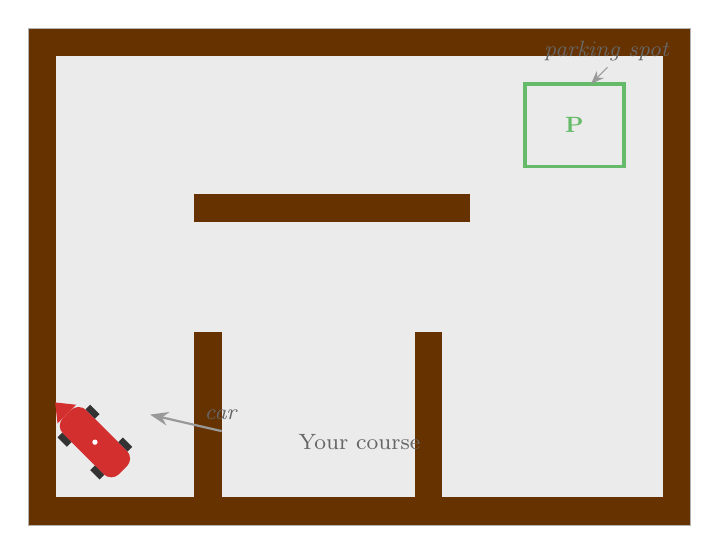
\begin{tikzpicture}[scale=0.7]
  % Stage outline
  \draw[black!30,thick] (-6,-4.5) rectangle (6,4.5);
  % Road surface
  \fill[roadgrey!30] (-6,-4.5) rectangle (6,4.5);
  % Walls
  \fill[wallbrown] (-6,-4.5) rectangle (-5.5,4.5);
  \fill[wallbrown] (5.5,-4.5) rectangle (6,4.5);
  \fill[wallbrown] (-6,4) rectangle (6,4.5);
  \fill[wallbrown] (-6,-4.5) rectangle (6,-4);
  % Inner walls
  \fill[wallbrown] (-3,-4) rectangle (-2.5,-1);
  \fill[wallbrown] (1,-4) rectangle (1.5,-1);
  \fill[wallbrown] (-3,1) rectangle (2,1.5);
  % Parking spot
  \draw[parkgreen,very thick] (3,2) rectangle (4.8,3.5);
  \node[parkgreen,font=\footnotesize\bfseries] at (3.9,2.75) {P};
  % Car
  \begin{scope}[scale=1.2]
    \drawcar{-4}{-2.5}{45}
  \end{scope}
  % Labels
  \node[font=\footnotesize,black!60] at (0,-3) {Your course};
  \draw[-{Stealth},black!40,thick] (-2.5,-2.8) -- (-3.8,-2.5);
  \node[font=\footnotesize,black!60] at (-2.5,-2.5) {\textit{car}};
  \draw[-{Stealth},black!40] (4.5,3.8) -- (4.2,3.5);
  \node[font=\footnotesize,black!60] at (4.5,4.1) {\textit{parking spot}};
\end{tikzpicture}
\end{center}

A top-down racing game where you steer a cigar-shaped race car around a course, avoid the walls, and park it perfectly in a parking spot. There's a timer, a crash counter, and a happy sound when you nail it.

Let's go.

\tableofcontents
\newpage

% =============================================
% SESSION 1
% =============================================
\section{Where Is My Car?}
\textit{\large Position and Direction}

\subsection{What We Already Know}

You've done coordinates before in maths --- like finding a square on a grid by going along and then up. ``3 across, 2 up'' --- that kind of thing.

You also know about turns. A quarter turn is a right angle (90 degrees). A half turn is 180 degrees. A full turn is 360 degrees --- you end up facing the same way you started.

That's actually most of what you need to know to place a car on a screen and point it in a direction.

\subsection{The New Idea: Position and Direction}

Everything in a game has two basic facts about it:

\begin{enumerate}
  \item \textbf{Position} --- \emph{where} it is
  \item \textbf{Direction} --- \emph{which way} it's facing
\end{enumerate}

Position is just two numbers: how far across (left--right) and how far up--down. In Scratch, these are called \textbf{x} and \textbf{y}.

\begin{center}
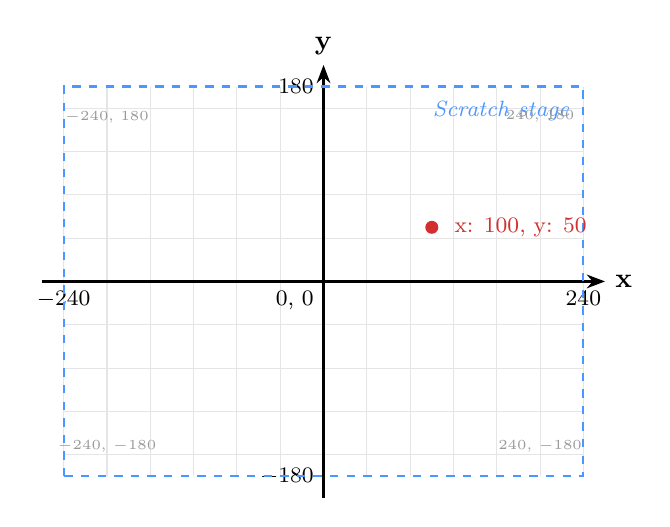
\begin{tikzpicture}[scale=0.55]
  % Grid
  \draw[black!10] (-6,-4.5) grid[step=1] (6,4.5);
  % Axes
  \draw[-{Stealth},thick] (-6.5,0) -- (6.5,0) node[right] {\textbf{x}};
  \draw[-{Stealth},thick] (0,-5) -- (0,5) node[above] {\textbf{y}};
  % Labels
  \node[below left,font=\footnotesize] at (0,0) {0, 0};
  \node[below,font=\footnotesize] at (6,0) {240};
  \node[below,font=\footnotesize] at (-6,0) {$-$240};
  \node[left,font=\footnotesize] at (0,4.5) {180};
  \node[left,font=\footnotesize] at (0,-4.5) {$-$180};
  % Stage border
  \draw[scratchblue,thick,dashed] (-6,-4.5) rectangle (6,4.5);
  \node[scratchblue,font=\footnotesize\itshape,anchor=north east] at (5.9,4.4) {Scratch stage};
  % Example point
  \fill[carred] (2.5,1.25) circle (0.15);
  \node[carred,font=\footnotesize,anchor=west] at (2.8,1.25) {x: 100, y: 50};
  % Corner labels
  \node[font=\tiny,black!40] at (-5,3.8) {$-$240, 180};
  \node[font=\tiny,black!40] at (5,3.8) {240, 180};
  \node[font=\tiny,black!40] at (-5,-3.8) {$-$240, $-$180};
  \node[font=\tiny,black!40] at (5,-3.8) {240, $-$180};
\end{tikzpicture}
\end{center}

Direction is an angle --- a number of degrees. In Scratch, direction works like a compass:

\begin{center}
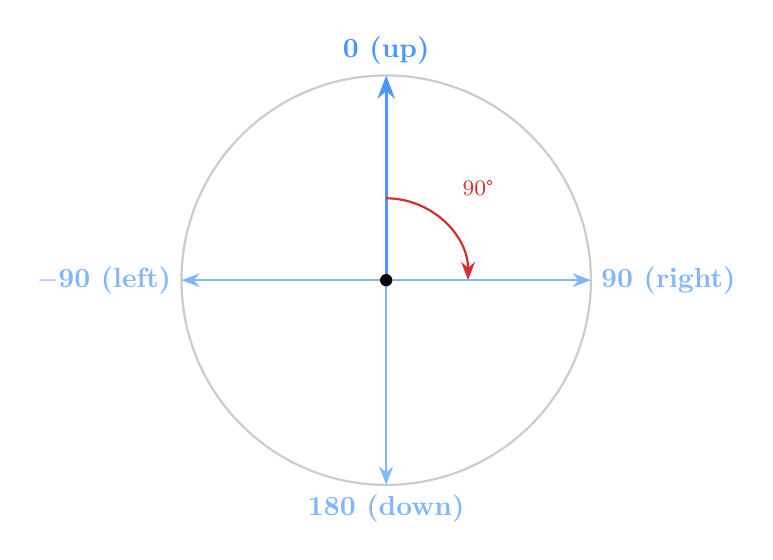
\begin{tikzpicture}[scale=1.3]
  % Circle
  \draw[black!20,thick] (0,0) circle (2);
  % Directions
  \draw[-{Stealth},scratchblue,very thick] (0,0) -- (0,2) node[above,font=\bfseries] {0 (up)};
  \draw[-{Stealth},scratchblue!70,thick] (0,0) -- (2,0) node[right,font=\bfseries] {90 (right)};
  \draw[-{Stealth},scratchblue!70,thick] (0,0) -- (0,-2) node[below,font=\bfseries] {180 (down)};
  \draw[-{Stealth},scratchblue!70,thick] (0,0) -- (-2,0) node[left,font=\bfseries] {$-$90 (left)};
  % Angle arc examples
  \draw[-{Stealth},carred,thick] (0,0.8) arc (90:0:0.8);
  \node[carred,font=\footnotesize] at (0.9,0.9) {90\textdegree};
  % Centre
  \fill[black] (0,0) circle (0.06);
\end{tikzpicture}
\end{center}

So if your car is at x: 100, y: 50 and its direction is 90, it's sitting in the right half of the screen, pointing to the right.

\begin{parentbox}
Scratch's direction system is like a compass --- 0 is north (up). This matches what children learn about compass directions in Year~3 geography. The x/y system maps directly to the coordinate grids they've used in maths, though Scratch extends into negative numbers. If your child hasn't met negatives yet, just say ``minus means the other way'' --- left instead of right, or down instead of up.
\end{parentbox}

\subsection{Let's Build It}

\subsubsection{Step 1: Create a new project}

Open Scratch and click ``Create''. You'll see the cat sprite on the stage. We don't need the cat --- right-click on it and choose ``delete''.

\subsubsection{Step 2: Draw your car}

Click the paintbrush icon (``Paint'') to create a new sprite. We're going to draw a top-down racing car --- a long, thin shape like an old-fashioned cigar-shaped race car.

\begin{center}
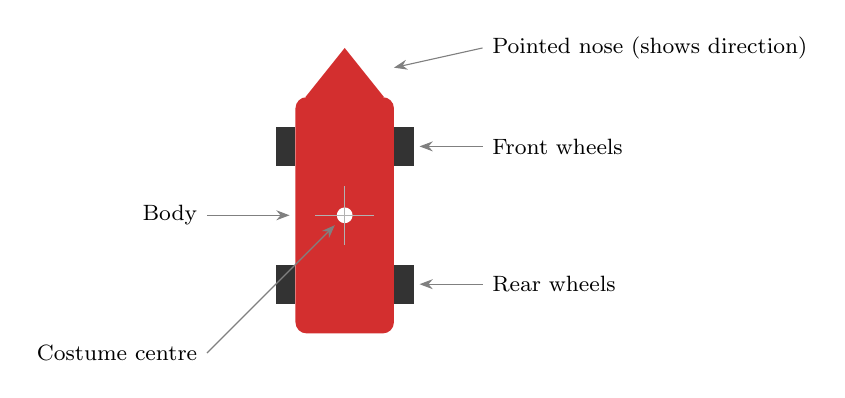
\begin{tikzpicture}[scale=2.5]
  \drawcar{0}{0}{0}
  % Annotations
  \draw[-{Stealth},black!50] (0.7,0.85) -- (0.25,0.75);
  \node[font=\footnotesize,anchor=west] at (0.7,0.85) {Pointed nose (shows direction)};
  \draw[-{Stealth},black!50] (0.7,0.35) -- (0.38,0.35);
  \node[font=\footnotesize,anchor=west] at (0.7,0.35) {Front wheels};
  \draw[-{Stealth},black!50] (0.7,-0.35) -- (0.38,-0.35);
  \node[font=\footnotesize,anchor=west] at (0.7,-0.35) {Rear wheels};
  \draw[-{Stealth},black!50] (-0.7,0) -- (-0.28,0);
  \node[font=\footnotesize,anchor=east] at (-0.7,0) {Body};
  % Centre crosshair
  \draw[black!30,thin] (-0.15,0) -- (0.15,0);
  \draw[black!30,thin] (0,-0.15) -- (0,0.15);
  \draw[-{Stealth},black!50] (-0.7,-0.7) -- (-0.05,-0.05);
  \node[font=\footnotesize,anchor=east] at (-0.7,-0.7) {Costume centre};
\end{tikzpicture}
\end{center}

\begin{enumerate}
  \item Select the \textbf{oval tool} and draw a long, narrow oval in red (about 3 times taller than wide)
  \item Add a small \textbf{triangle} at the top --- the pointed nose that shows which way the car faces
  \item Add four small \textbf{rectangles} for wheels (two at the back, two at the front)
  \item Make sure the car points \textbf{up} (Scratch's default direction is 0 = up)
\end{enumerate}

\begin{parentbox}
The car's ``costume centre'' (the crosshair in the costume editor) should be in the middle of the car body. This is the point it rotates around. If it's off-centre, the car will wobble when it turns. Drag the costume to adjust this.
\end{parentbox}

\subsubsection{Step 3: Add movement code}

Click on your car sprite, then go to the Code tab. Build this script:

\begin{scratchblockbox}
\begin{lstlisting}[style=scratch]
when green flag clicked
go to x: (0) y: (0)
point in direction (0)
forever
  if <key [up arrow] pressed?> then
    move (3) steps
  end
  if <key [down arrow] pressed?> then
    move (-3) steps
  end
  if <key [left arrow] pressed?> then
    turn left (3) degrees
  end
  if <key [right arrow] pressed?> then
    turn right (3) degrees
  end
end
\end{lstlisting}
\end{scratchblockbox}

\textbf{Where to find these blocks:}
\begin{itemize}[nosep]
  \item \texttt{when green flag clicked} --- \textbf{Events} (yellow)
  \item \texttt{go to x: y:} and \texttt{point in direction} --- \textbf{Motion} (blue)
  \item \texttt{forever}, \texttt{if then} --- \textbf{Control} (orange)
  \item \texttt{key pressed?} --- \textbf{Sensing} (light blue)
  \item \texttt{move} and \texttt{turn} --- \textbf{Motion} (blue)
\end{itemize}

\subsubsection{Step 4: Try it!}

Click the green flag. Use the arrow keys to drive around. \textbf{Up} moves forward, \textbf{Down} moves backward, \textbf{Left} and \textbf{Right} spin the car.

You've built the most basic driving game possible. The car knows \emph{where} it is and \emph{which way} it's facing, and you can change both.

\begin{challengebox}
\begin{itemize}[nosep]
  \item Drive to each corner of the stage
  \item Try to drive in a straight line from left to right (hint: point the car to direction 90 first)
  \item Park on the exact centre (x:~0, y:~0) --- check the x and y values below the stage
\end{itemize}
\end{challengebox}

\begin{stretchbox}
Draw a road on the \textbf{backdrop}. Click the stage, then the ``Backdrops'' tab, and use the rectangle tool to draw grey roads on a green background. Now your car has somewhere to drive!
\end{stretchbox}

\newpage

% =============================================
% SESSION 2
% =============================================
\section{Fast and Slow}
\textit{\large Speed, acceleration, and braking}

\subsection{What We Already Know}

You know about measuring distances --- centimetres, metres, kilometres. You know that some things are fast (a cheetah) and some things are slow (a snail). And you know from maths that bigger numbers mean more: 10 steps takes you further than 3 steps.

\subsection{The New Idea: Speed}

In Session~1, our car moved 3 steps every time. Real cars don't work like that. Real cars:

\begin{itemize}[nosep]
  \item \textbf{Speed up gradually} when you press the accelerator
  \item \textbf{Slow down gradually} when you let go
  \item \textbf{Brake} when you press the brake
  \item \textbf{Coast} to a stop --- they don't stop instantly
\end{itemize}

\textbf{Speed} is just a number: ``how far does the car move each moment?'' If speed is 0, the car is still. If speed is 5, it zips along. If speed is $-2$, it goes backward.

\begin{center}
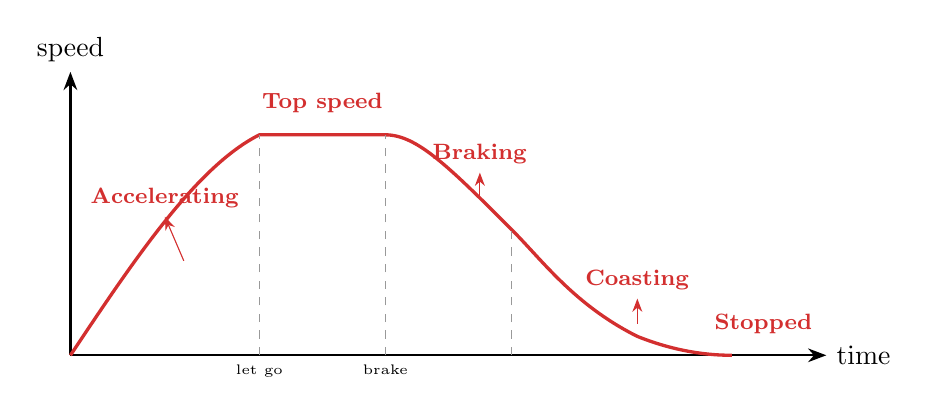
\begin{tikzpicture}[scale=0.8]
  % Timeline
  \draw[-{Stealth},thick] (0,0) -- (12,0) node[right] {time};
  \draw[-{Stealth},thick] (0,0) -- (0,4.5) node[above] {speed};
  % Speed curve
  \draw[carred,very thick]
    (0,0)
    .. controls (1,1.5) and (2,3) .. (3,3.5)
    -- (5,3.5)
    .. controls (5.5,3.5) and (6,3) .. (7,2)
    .. controls (7.5,1.5) and (8,0.8) .. (9,0.3)
    .. controls (9.5,0.1) and (10,0) .. (10.5,0);
  % Labels
  \node[font=\footnotesize,carred] at (1.5,2.5) {\textbf{Accelerating}};
  \draw[{Stealth}-,carred] (1.5,2.2) -- (1.8,1.5);
  \node[font=\footnotesize,carred] at (4,4) {\textbf{Top speed}};
  \node[font=\footnotesize,carred] at (6.5,3.2) {\textbf{Braking}};
  \draw[{Stealth}-,carred] (6.5,2.9) -- (6.5,2.5);
  \node[font=\footnotesize,carred] at (9,1.2) {\textbf{Coasting}};
  \draw[{Stealth}-,carred] (9,0.9) -- (9,0.5);
  \node[font=\footnotesize,carred] at (11,0.5) {\textbf{Stopped}};
  % Annotations
  \draw[black!40,dashed] (3,0) -- (3,3.5);
  \draw[black!40,dashed] (5,0) -- (5,3.5);
  \draw[black!40,dashed] (7,0) -- (7,2);
  \node[font=\tiny,below] at (3,0) {let go};
  \node[font=\tiny,below] at (5,0) {brake};
\end{tikzpicture}
\end{center}

\textbf{Acceleration} changes the speed. Press the accelerator, speed goes up. Brake, speed goes down.

\textbf{Friction} slows you down even when you're not braking. The road and air resistance drag on the car. In our game, we shrink the speed by 5\% each moment, so the car naturally coasts to a stop.

\begin{parentbox}
We're keeping this intuitive --- speed as ``steps per frame,'' acceleration as ``speed change per frame.'' Friction is simplified to a multiplier (\texttt{speed $\times$ 0.95} each frame), which mimics drag well for a game. The formal $v = d/t$ and the distinction between static and kinetic friction aren't needed here --- the key insight is just ``things slow down on their own.''
\end{parentbox}

\subsection{Let's Build It}

\subsubsection{Step 1: Create a speed variable}

Go to \textbf{Variables} (orange) and click ``Make a Variable''. Call it \texttt{speed}. Select ``For this sprite only''.

\subsubsection{Step 2: Update the movement code}

Replace your old script with this:

\begin{scratchblockbox}
\begin{lstlisting}[style=scratch]
when green flag clicked
go to x: (0) y: (0)
point in direction (0)
set [speed] to (0)
forever
  if <key [up arrow] pressed?> then
    change [speed] by (0.3)
  end
  if <key [down arrow] pressed?> then
    change [speed] by (-0.5)
  end
  if <key [left arrow] pressed?> then
    turn left (3) degrees
  end
  if <key [right arrow] pressed?> then
    turn right (3) degrees
  end
  move (speed) steps
  set [speed] to ((speed) * (0.95))
end
\end{lstlisting}
\end{scratchblockbox}

\textbf{What changed:}
\begin{itemize}[nosep]
  \item \texttt{speed} starts at 0 (car begins stationary)
  \item Up arrow increases \texttt{speed} by 0.3 (gentle acceleration)
  \item Down arrow decreases \texttt{speed} by 0.5 (braking is stronger --- like a real car)
  \item \texttt{move (speed) steps} --- the car moves by the current speed
  \item \texttt{speed $\times$ 0.95} --- \textbf{friction!} Speed shrinks 5\% each frame, so the car coasts to a stop
\end{itemize}

\begin{center}
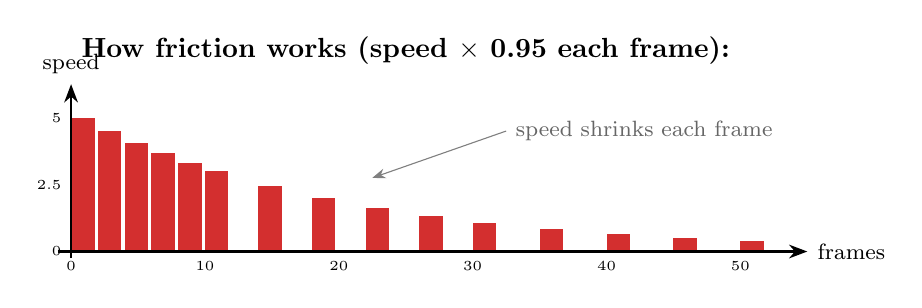
\begin{tikzpicture}[scale=0.85]
  \node[font=\bfseries] at (5,3) {How friction works (speed $\times$ 0.95 each frame):};
  % Decay bars - wider and more visible
  \foreach \i/\v in {0/5.00, 2/4.51, 4/4.07, 6/3.67, 8/3.31, 10/2.99, 14/2.44, 18/1.99, 22/1.62, 26/1.32, 30/1.07, 35/0.83, 40/0.64, 45/0.50, 50/0.38} {
    \pgfmathsetmacro{\x}{\i * 0.2}
    \fill[carred] (\x,0) rectangle (\x+0.35,\v/5*2);
  }
  \draw[-{Stealth},thick] (-0.2,0) -- (11,0) node[right,font=\footnotesize] {frames};
  \draw[-{Stealth},thick] (0,-0.1) -- (0,2.5) node[above,font=\footnotesize] {speed};
  \node[font=\tiny,below] at (0,0) {0};
  \node[font=\tiny,below] at (2,0) {10};
  \node[font=\tiny,below] at (4,0) {20};
  \node[font=\tiny,below] at (6,0) {30};
  \node[font=\tiny,below] at (8,0) {40};
  \node[font=\tiny,below] at (10,0) {50};
  % Speed labels
  \node[font=\tiny,left] at (0,2) {5};
  \node[font=\tiny,left] at (0,1) {2.5};
  \node[font=\tiny,left] at (0,0) {0};
  % Annotation
  \draw[-{Stealth},black!50] (6.5,1.8) -- (4.5,1.1);
  \node[font=\footnotesize,black!60,anchor=west] at (6.5,1.8) {speed shrinks each frame};
\end{tikzpicture}
\end{center}

\subsubsection{Step 3: Add a speed limit}

Cars can't go infinitely fast. Add this inside the \texttt{forever} loop, after the key checks but before \texttt{move}:

\begin{scratchblockbox}
\begin{lstlisting}[style=scratch]
if <(speed) > (5)> then
  set [speed] to (5)
end
if <(speed) < (-3)> then
  set [speed] to (-3)
end
\end{lstlisting}
\end{scratchblockbox}

This caps forward speed at 5 and reverse at 3 (reversing is always slower).

\begin{parentbox}
The \texttt{$\times$ 0.95} is the key physics trick. Speed decays exponentially --- fast speeds drop quickly, slow speeds linger. If your child asks ``why 0.95?'', try changing it: 0.8 = lots of friction (like sand), 0.99 = almost none (like ice). Great way to build intuition.
\end{parentbox}

\begin{challengebox}
\begin{itemize}[nosep]
  \item Accelerate to top speed, then let go. How far does the car coast?
  \item Try to stop on an exact spot --- it's harder now!
  \item Hold down arrow while moving forward --- feel how braking works
  \item What happens if you hold down arrow when stopped? (It reverses!)
\end{itemize}
\end{challengebox}

\begin{stretchbox}
Make the \texttt{speed} variable visible on stage (tick its checkbox). Instant speedometer! For a fancier one, create a bar sprite whose size follows the speed value.
\end{stretchbox}

\newpage

% =============================================
% SESSION 3
% =============================================
\section{Turning the Wheel}
\textit{\large Steering and turning radius}

\subsection{What We Already Know}

You know about turns --- quarter turns (right angles), half turns, full turns. You know that turning the steering wheel makes the front wheels point left or right, and that's what makes a car turn.

Here's something you might have noticed: if a car is standing still and you turn the steering wheel, the car doesn't go anywhere. The wheels just point sideways. The car only \emph{actually turns} when it's moving.

\subsection{The New Idea: Steering and Turning Radius}

\textbf{How fast you're going changes how sharply you can turn.}

Think about riding a bicycle:
\begin{itemize}[nosep]
  \item Going \textbf{slowly}: you can turn really tightly, almost spinning on the spot
  \item Going \textbf{fast}: you have to make a big, wide turn
  \item \textbf{Standing still}: you can turn the handlebars but the bike doesn't change direction
\end{itemize}

\begin{center}
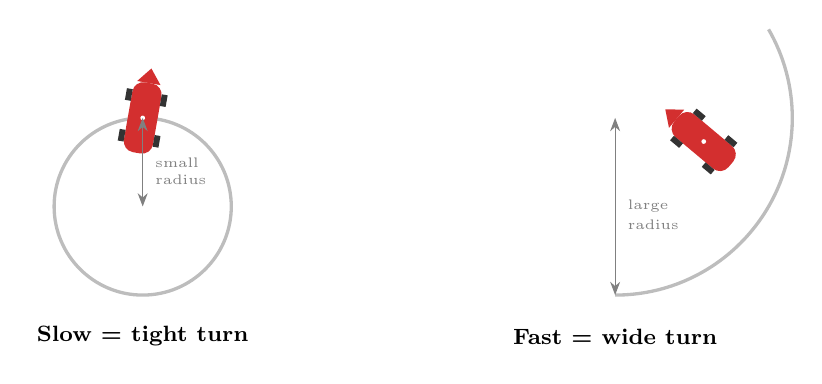
\begin{tikzpicture}[scale=0.75]
  % Slow turn (tight)
  \begin{scope}[shift={(-4,0)}]
    \draw[roadgrey,very thick] (0,0) circle (1.5);
    \drawcar{0}{1.5}{-10}
    \node[font=\footnotesize\bfseries] at (0,-2.2) {Slow = tight turn};
    \draw[{Stealth}-{Stealth},black!50] (0,0) -- (0,1.5);
    \node[font=\tiny,black!50,right] at (0.05,0.75) {small};
    \node[font=\tiny,black!50,right] at (0.05,0.45) {radius};
  \end{scope}
  % Fast turn (wide)
  \begin{scope}[shift={(4,0)}]
    \draw[roadgrey,very thick] (0,-1.5) arc (-90:30:3);
    \drawcar{1.5}{1.1}{50}
    \node[font=\footnotesize\bfseries] at (0,-2.2) {Fast = wide turn};
    \draw[{Stealth}-{Stealth},black!50] (0,-1.5) -- (0,1.5);
    \node[font=\tiny,black!50,right] at (0.05,0) {large};
    \node[font=\tiny,black!50,right] at (0.05,-0.3) {radius};
  \end{scope}
\end{tikzpicture}
\end{center}

This is called the \textbf{turning radius}. Slow = tight turns. Fast = wide turns.

This is exactly why parking needs slow speed. You need tight turns to fit into a space, and you can only make tight turns when you're going slowly.

\begin{parentbox}
The real physics involves the relationship between velocity, steering angle, and the resulting circular arc ($R = L / \tan(\theta)$ where $L$ is wheelbase length). We simplify to ``turning amount scales with speed,'' which captures the essential insight. The key idea --- that turning effectiveness depends on forward motion --- is genuinely important and often surprises children and adults alike.
\end{parentbox}

\subsection{Let's Build It}

\subsubsection{Step 1: Create a steering variable}

Make a new variable called \texttt{steering} (for this sprite only). It represents the steering wheel position: negative = left, positive = right, zero = straight.

\subsubsection{Step 2: Update the steering code}

Replace the left/right arrow handling and the turn line:

\begin{scratchblockbox}
\begin{lstlisting}[style=scratch]
set [steering] to (0)
  ...inside forever loop...
  if <key [left arrow] pressed?> then
    set [steering] to (-5)
  else
    if <key [right arrow] pressed?> then
      set [steering] to (5)
    else
      set [steering] to (0)
    end
  end
  turn right ((steering) * ((speed) / (3))) degrees
\end{lstlisting}
\end{scratchblockbox}

\textbf{The key line:} \texttt{turn right ((steering) $\times$ ((speed) / (3))) degrees}

This means: turn by the steering amount, multiplied by how fast you're going.

\begin{center}
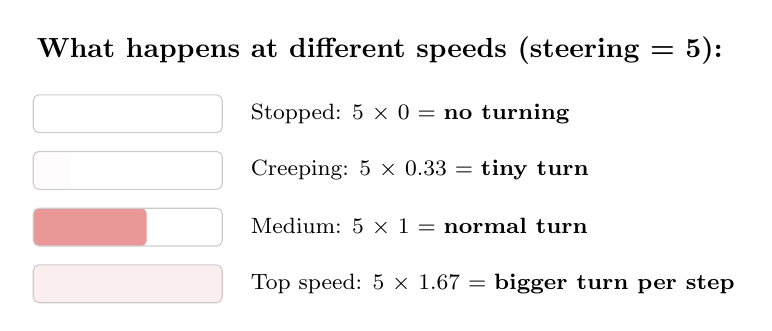
\begin{tikzpicture}[scale=0.8]
  % Table-like display
  \node[font=\bfseries] at (0,3) {What happens at different speeds (steering = 5):};
  \foreach \s/\v/\r/\label in {
    0/0/0/{Stopped: 5 $\times$ 0 = \textbf{no turning}},
    1/1/1.67/{Creeping: 5 $\times$ 0.33 = \textbf{tiny turn}},
    2/3/5/{Medium: 5 $\times$ 1 = \textbf{normal turn}},
    3/5/8.33/{Top speed: 5 $\times$ 1.67 = \textbf{bigger turn per step}}%
  } {
    \pgfmathsetmacro{\y}{2 - \s * 0.9}
    \fill[carred!\r0!white,rounded corners=2pt] (-5.5,\y-0.3) rectangle (-5.5+\r/8.33*3,\y+0.3);
    \draw[black!20,rounded corners=2pt] (-5.5,\y-0.3) rectangle (-2.5,\y+0.3);
    \node[font=\footnotesize,anchor=west] at (-2.2,\y) {\label};
  }
\end{tikzpicture}
\end{center}

\subsubsection{Step 3: Add a wheel indicator}

Create three costumes for your car:

\begin{center}
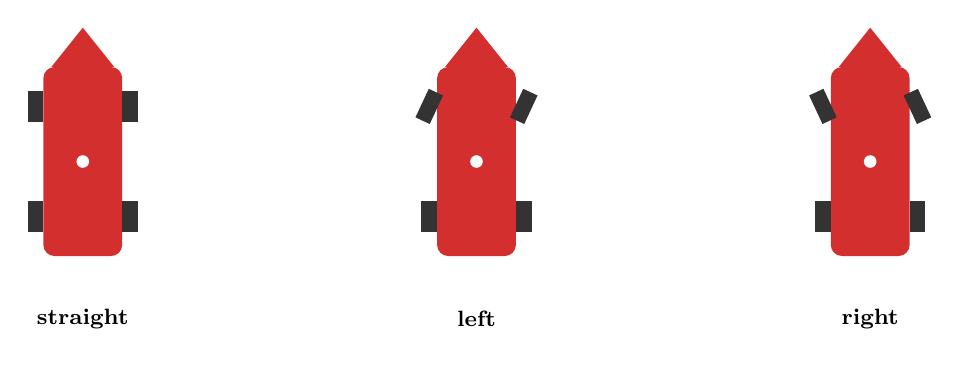
\begin{tikzpicture}[scale=2]
  % Straight
  \drawcar{-2.5}{0}{0}
  \node[font=\footnotesize\bfseries] at (-2.5,-1) {straight};
  % Left
  \drawcarsteered{0}{0}{0}{-25}
  \node[font=\footnotesize\bfseries] at (0,-1) {left};
  % Right
  \drawcarsteered{2.5}{0}{0}{25}
  \node[font=\footnotesize\bfseries] at (2.5,-1) {right};
\end{tikzpicture}
\end{center}

Add this inside the \texttt{forever} loop:

\begin{scratchblockbox}
\begin{lstlisting}[style=scratch]
if <(steering) < (0)> then
  switch costume to [left]
else
  if <(steering) > (0)> then
    switch costume to [right]
  else
    switch costume to [straight]
  end
end
\end{lstlisting}
\end{scratchblockbox}

Now you can see the wheels turn when you steer!

\begin{challengebox}
\begin{itemize}[nosep]
  \item Drive in a circle at slow speed. Now try at top speed --- what happens?
  \item Try to drive in a perfect square: forward, right angle turn, forward\ldots{} (slow down for corners!)
  \item Coast forward and steer --- the turning gets tighter as you slow down!
\end{itemize}
\end{challengebox}

\begin{stretchbox}
Try changing the steering value from 5 to 8 or 3. Racing drivers call this ``steering sensitivity'' --- find what feels best for your game.
\end{stretchbox}

\newpage

% =============================================
% SESSION 4
% =============================================
\section{Walls and Bumps}
\textit{\large Collision detection}

\subsection{What We Already Know}

In science, you've learned about \textbf{forces} --- pushes and pulls. When you push a toy car into a wall, the wall pushes back. The car stops. Two solid things can't be in the same place at the same time.

\subsection{The New Idea: Collision}

A \textbf{collision} is when two objects touch or overlap. In our game, we check every single frame: ``is the car touching a wall?'' If so:

\begin{enumerate}
  \item \textbf{Push back} to the last safe position
  \item \textbf{Stop} (set speed to 0)
  \item \textbf{Bonk!} (play a bump sound)
\end{enumerate}

\begin{center}
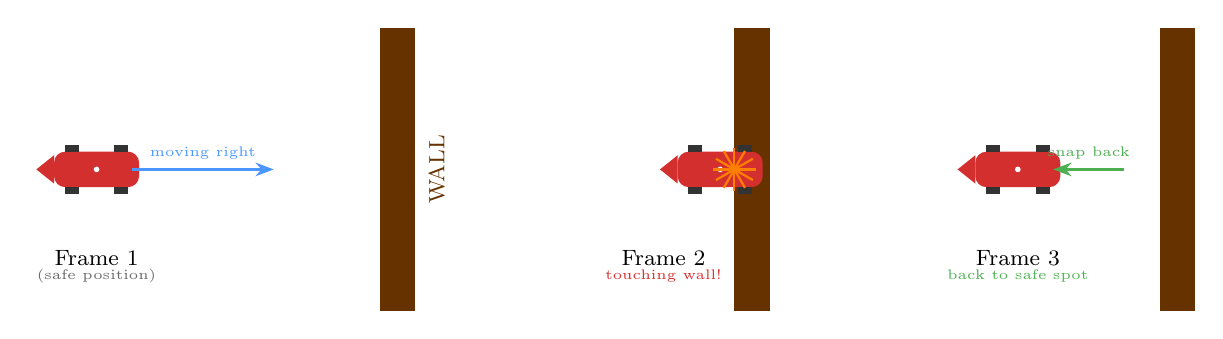
\begin{tikzpicture}[scale=0.9]
  % Wall
  \fill[wallbrown] (2,-2) rectangle (2.5,2);
  \node[font=\footnotesize,wallbrown,rotate=90] at (2.8,0) {WALL};

  % Frame 1: before
  \begin{scope}[shift={(-2,0)}]
    \drawcar{0}{0}{90}
    \node[font=\footnotesize,below] at (0,-1) {Frame 1};
    \node[font=\tiny,black!60] at (0,-1.5) {(safe position)};
    \draw[-{Stealth},scratchblue,thick] (0.5,0) -- (2.5,0);
    \node[font=\tiny,scratchblue,above] at (1.5,0) {moving right};
  \end{scope}

  % Frame 2: touching wall
  \begin{scope}[shift={(5,0)}]
    \fill[wallbrown] (2,-2) rectangle (2.5,2);
    \drawcar{1.8}{0}{90}
    \node[font=\footnotesize,below] at (1,-1) {Frame 2};
    \node[font=\tiny,carred] at (1,-1.5) {touching wall!};
    % Collision star
    \foreach \a in {0,30,...,330} {
      \draw[orange,thick] (2,0) -- +(\a:0.3);
    }
  \end{scope}

  % Frame 3: pushed back
  \begin{scope}[shift={(11,0)}]
    \fill[wallbrown] (2,-2) rectangle (2.5,2);
    \drawcar{0}{0}{90}
    \node[font=\footnotesize,below] at (0,-1) {Frame 3};
    \node[font=\tiny,grassgreen] at (0,-1.5) {back to safe spot};
    \draw[-{Stealth},grassgreen,thick] (1.5,0) -- (0.5,0);
    \node[font=\tiny,grassgreen,above] at (1,0) {snap back};
  \end{scope}
\end{tikzpicture}
\end{center}

\begin{parentbox}
Real game physics engines use sophisticated collision detection (separating axis theorem, impulse resolution). In Scratch, we use colour-based collision, which is simpler but works well. The ``push back'' is important --- without it, the car gets stuck inside the wall. We remember the last safe position and snap back to it each time a collision is detected.
\end{parentbox}

\subsection{Let's Build It}

\subsubsection{Step 1: Design the course}

Click on the \textbf{Stage}, then the \textbf{Backdrops} tab. Draw a course:
\begin{enumerate}[nosep]
  \item Fill the backdrop with \textbf{light grey} (road)
  \item Use \textbf{dark brown} (\texttt{\#663300}) to draw walls: border walls and some inner walls to create corridors
  \item Leave a clear starting area and a path to where the parking spot will go
\end{enumerate}

\begin{center}
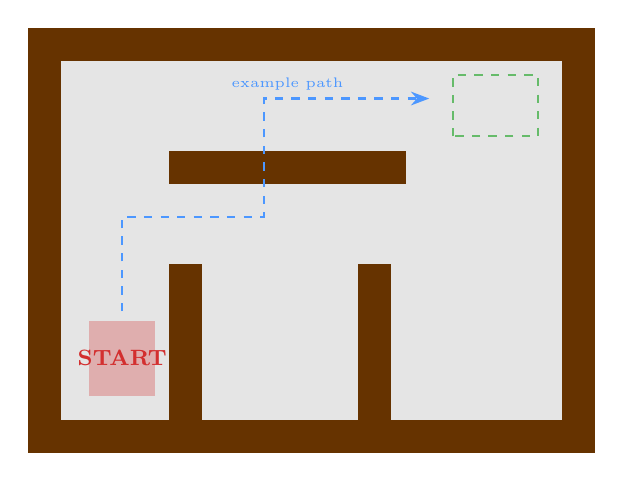
\begin{tikzpicture}[scale=0.6]
  % Road
  \fill[roadgrey!40] (-6,-4.5) rectangle (6,4.5);
  % Border walls
  \fill[wallbrown] (-6,-4.5) rectangle (-5.3,4.5);
  \fill[wallbrown] (5.3,-4.5) rectangle (6,4.5);
  \fill[wallbrown] (-6,3.8) rectangle (6,4.5);
  \fill[wallbrown] (-6,-4.5) rectangle (6,-3.8);
  % Inner walls
  \fill[wallbrown] (-3,-3.8) rectangle (-2.3,-0.5);
  \fill[wallbrown] (1,-3.8) rectangle (1.7,-0.5);
  \fill[wallbrown] (-3,1.2) rectangle (2,1.9);
  % Parking spot (preview)
  \draw[parkgreen,thick,dashed] (3,2.2) rectangle (4.8,3.5);
  % Start
  \node[font=\footnotesize\bfseries,carred] at (-4,-2.5) {START};
  \fill[carred,opacity=0.3] (-4.7,-3.3) rectangle (-3.3,-1.7);
  % Path arrows
  \draw[-{Stealth},scratchblue,thick,dashed] (-4,-1.5) -- (-4,0.5) -- (-1,0.5) -- (-1,3) -- (2.5,3);
  \node[font=\tiny,scratchblue] at (-0.5,3.3) {example path};
\end{tikzpicture}
\end{center}

\textbf{Important:} Use \emph{one specific colour} for all walls. We detect this colour to know when the car has hit a wall.

\subsubsection{Step 2: Add position memory}

Create two new variables (for this sprite only):
\begin{itemize}[nosep]
  \item \texttt{last x}
  \item \texttt{last y}
\end{itemize}

\subsubsection{Step 3: Update the code}

Add these lines to your car's \texttt{forever} loop. \textbf{Before} any movement:

\begin{scratchblockbox}
\begin{lstlisting}[style=scratch]
set [last x] to (x position)
set [last y] to (y position)
\end{lstlisting}
\end{scratchblockbox}

\textbf{After} the \texttt{move} block, add collision detection:

\begin{scratchblockbox}
\begin{lstlisting}[style=scratch]
if <touching color (#663300)?> then
  go to x: (last x) y: (last y)
  set [speed] to (0)
  start sound [Boing]
end
\end{lstlisting}
\end{scratchblockbox}

This checks: ``Am I touching the wall colour?'' If yes: snap back, stop, bonk.

\begin{parentbox}
To pick the right colour in the \texttt{touching color} block, click the colour swatch, then click the eyedropper tool, then click on the wall colour on your backdrop. The ``Boing'' sound is in Scratch's sound library --- go to the Sounds tab and click the speaker icon to browse and add it.
\end{parentbox}

Also change the starting position to somewhere sensible on your course:

\begin{scratchblockbox}
\begin{lstlisting}[style=scratch]
go to x: (-180) y: (-120)
\end{lstlisting}
\end{scratchblockbox}

\begin{challengebox}
\begin{itemize}[nosep]
  \item Drive the full course without hitting a single wall
  \item Try hitting a wall at top speed vs.\ low speed
  \item Find the tightest corner. Can you get around it? (Remember: slow = tight turns!)
\end{itemize}
\end{challengebox}

\begin{stretchbox}
Add a crash counter! Create a \texttt{crashes} variable (for all sprites). Set it to 0 on green flag. Inside the collision \texttt{if} block, add \texttt{change [crashes] by (1)}. Can you finish the course with zero crashes?
\end{stretchbox}

\newpage

% =============================================
% SESSION 5
% =============================================
\section{Park It!}
\textit{\large The parking challenge}

\subsection{What We Already Know}

You've fitted shapes into spaces before --- jigsaw puzzles, shape sorters, tidying a shelf. You know that to fit something into a space, it needs to be the right size, in the right place, and pointing the right way.

\subsection{The New Idea: Parking as a Physics Puzzle}

Parking is hard because you need \textbf{three things right at the same time:}

\begin{center}
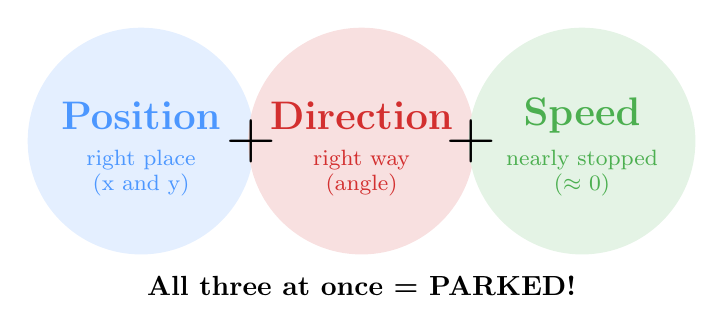
\begin{tikzpicture}[scale=0.8]
  % Three circles
  \fill[scratchblue!15] (-3.5,0) circle (1.8);
  \fill[carred!15] (0,0) circle (1.8);
  \fill[grassgreen!15] (3.5,0) circle (1.8);
  % Labels
  \node[font=\Large\bfseries,scratchblue] at (-3.5,0.4) {Position};
  \node[font=\footnotesize,scratchblue] at (-3.5,-0.3) {right place};
  \node[font=\footnotesize,scratchblue] at (-3.5,-0.7) {(x and y)};

  \node[font=\Large\bfseries,carred] at (0,0.4) {Direction};
  \node[font=\footnotesize,carred] at (0,-0.3) {right way};
  \node[font=\footnotesize,carred] at (0,-0.7) {(angle)};

  \node[font=\Large\bfseries,grassgreen] at (3.5,0.4) {Speed};
  \node[font=\footnotesize,grassgreen] at (3.5,-0.3) {nearly stopped};
  \node[font=\footnotesize,grassgreen] at (3.5,-0.7) {($\approx$ 0)};

  % Plus signs
  \node[font=\Huge] at (-1.75,0) {+};
  \node[font=\Huge] at (1.75,0) {+};

  % All three
  \node[font=\bfseries] at (0,-2.3) {All three at once = PARKED!};
\end{tikzpicture}
\end{center}

Each one on its own is easy. But doing all three \emph{together} --- that's the challenge. And because you can only turn well at low speed (Session~3), you have to do the hard part at exactly the speed where your controls are most sensitive.

That's why even grown-ups find parking tricky!

\begin{parentbox}
This connects to the mathematical idea of \emph{degrees of freedom}. The car has three variables to satisfy simultaneously (x, y, angle), which is what makes parking a challenging control problem. You might mention that real self-driving cars find parking one of the hardest tasks too!
\end{parentbox}

\subsection{Let's Build It}

\subsubsection{Step 1: Create the parking spot}

Create a new sprite (paintbrush icon). Draw a rectangle \textbf{outline only} --- no fill. Use bright \textbf{green} or \textbf{yellow}. Size it so the car just barely fits inside with a little room to spare.

Name this sprite ``ParkingSpot'' and position it:

\begin{scratchblockbox}
\begin{lstlisting}[style=scratch]
when green flag clicked
go to x: (150) y: (100)
point in direction (0)
\end{lstlisting}
\end{scratchblockbox}

\begin{center}
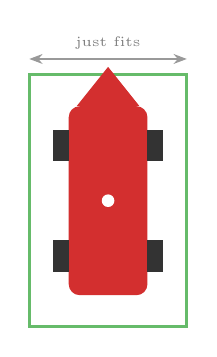
\begin{tikzpicture}[scale=2]
  % Parking spot
  \draw[parkgreen,very thick] (-0.5,-0.8) rectangle (0.5,0.8);
  % Car inside (good)
  \drawcar{0}{0}{0}
  % Arrows showing tight fit
  \draw[{Stealth}-{Stealth},black!40] (-0.5,0.9) -- (0.5,0.9);
  \node[font=\tiny,black!50,above] at (0,0.9) {just fits};
\end{tikzpicture}
\end{center}

\subsubsection{Step 2: Add parking detection}

Add this script to the \textbf{ParkingSpot} sprite:

\begin{scratchblockbox}
\begin{lstlisting}[style=scratch]
when green flag clicked
go to x: (150) y: (100)
point in direction (0)
set [parked] to (0)
forever
  if <<touching [Car]?> and
      <([speed] of [Car]) < (0.5)>> then
    if <<([speed] of [Car]) > (-0.5)> and
        <((abs of (([direction] of [Car]) - (0))) < (20))>> then
      set [parked] to (1)
      start sound [Collect]
      say [Parked!] for (2) seconds
      stop [all]
    end
  end
end
\end{lstlisting}
\end{scratchblockbox}

That's a lot of conditions! Here's what each one checks:

\begin{center}
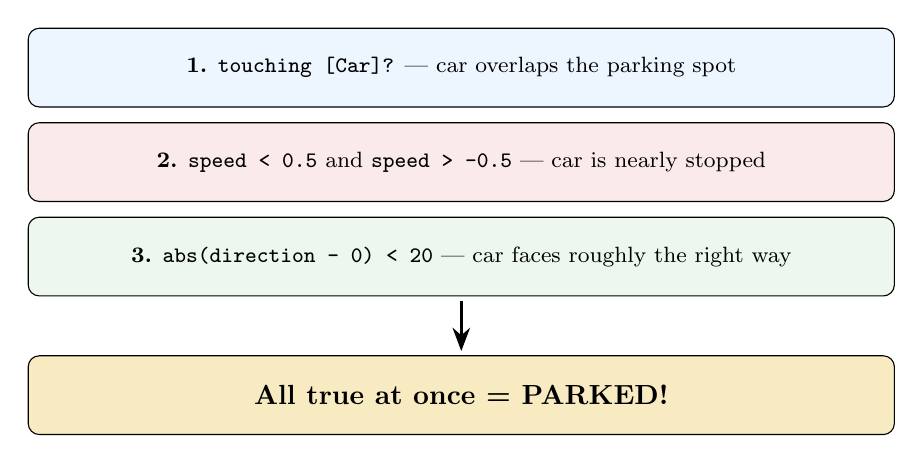
\begin{tikzpicture}[scale=0.8]
  \node[draw,rounded corners,fill=scratchblue!10,minimum width=11cm,minimum height=1cm,font=\footnotesize] at (0,3) {\textbf{1.} \texttt{touching [Car]?} --- car overlaps the parking spot};
  \node[draw,rounded corners,fill=carred!10,minimum width=11cm,minimum height=1cm,font=\footnotesize] at (0,1.5) {\textbf{2.} \texttt{speed < 0.5} and \texttt{speed > -0.5} --- car is nearly stopped};
  \node[draw,rounded corners,fill=grassgreen!10,minimum width=11cm,minimum height=1cm,font=\footnotesize] at (0,0) {\textbf{3.} \texttt{abs(direction - 0) < 20} --- car faces roughly the right way};
  \draw[very thick,-{Stealth}] (0,-0.7) -- (0,-1.5);
  \node[draw,rounded corners,fill=parentframe!30,minimum width=11cm,minimum height=1cm,font=\bfseries] at (0,-2.2) {All true at once = PARKED!};
\end{tikzpicture}
\end{center}

\begin{parentbox}
The \texttt{abs} block is in the \textbf{Operators} category (green), under the dropdown that starts with ``sqrt''. If your child asks what ``abs'' means, say: ``it throws away the minus sign --- it tells us how far from zero, whether plus or minus.'' The tolerance of 20 degrees is adjustable --- start generous, tighten later for more challenge.
\end{parentbox}

\subsubsection{Step 3: Add a happy sound}

On the ParkingSpot sprite, go to the \textbf{Sounds} tab, click the speaker icon, and add a celebratory sound --- ``Collect'', ``Win'', or ``Tada''.

\subsubsection{Step 4: Try it!}

Drive to the spot. Line up. Slow down. Match the angle. When all three conditions are met --- \textbf{PARKED!} Happy sound, message, game stops.

This is the moment. This is what we've been building towards.

\begin{challengebox}
\begin{itemize}[nosep]
  \item Park the car. How many attempts does it take?
  \item Try approaching from different angles --- which approach is easiest?
  \item Can you park with zero crashes?
  \item Try driving in fast --- the speed check stops you from ``cheating''!
\end{itemize}
\end{challengebox}

\begin{stretchbox}
Add a second parking spot in a trickier location --- maybe between two walls. Duplicate the ParkingSpot sprite and reposition it.
\end{stretchbox}

\newpage

% =============================================
% SESSION 6
% =============================================
\section{Make It a Real Game}
\textit{\large Polish, scoring, and the full experience}

\subsection{What We Already Know}

You know about counting and timing. You know what a ``personal best'' is. You know that the best games have a beginning, a middle, and an end.

Right now our game just\ldots{} starts. No ``ready, set, go.'' No score. No replay. Let's fix that.

\subsection{The New Idea: The Game Loop}

Every game follows a loop:

\begin{center}
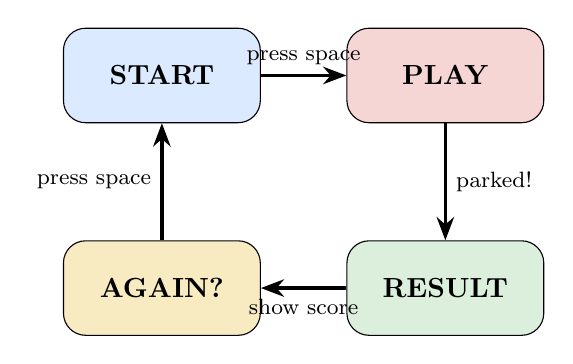
\begin{tikzpicture}[scale=0.9]
  \node[draw,rounded corners=8pt,fill=scratchblue!20,minimum width=2.5cm,minimum height=1.2cm,font=\bfseries] (start) at (0,2) {START};
  \node[draw,rounded corners=8pt,fill=carred!20,minimum width=2.5cm,minimum height=1.2cm,font=\bfseries] (play) at (4,2) {PLAY};
  \node[draw,rounded corners=8pt,fill=grassgreen!20,minimum width=2.5cm,minimum height=1.2cm,font=\bfseries] (end) at (4,-1) {RESULT};
  \node[draw,rounded corners=8pt,fill=parentframe!30,minimum width=2.5cm,minimum height=1.2cm,font=\bfseries] (again) at (0,-1) {AGAIN?};

  \draw[-{Stealth},very thick] (start) -- (play) node[midway,above,font=\footnotesize] {press space};
  \draw[-{Stealth},very thick] (play) -- (end) node[midway,right,font=\footnotesize] {parked!};
  \draw[-{Stealth},very thick] (end) -- (again) node[midway,below,font=\footnotesize] {show score};
  \draw[-{Stealth},very thick] (again) -- (start) node[midway,left,font=\footnotesize] {press space};
\end{tikzpicture}
\end{center}

This isn't physics --- it's \emph{game design}. But it's what turns a physics simulation into a game.

\begin{parentbox}
The game loop is a fundamental concept in computer science. Every game your child has played uses this pattern. The timer and crash counter together create a scoring tension --- speed vs.\ care --- which is what makes the game interesting and replayable.
\end{parentbox}

\subsection{Let's Build It}

\subsubsection{Step 1: Add a timer}

Scratch has a built-in timer. Add to the car's setup (right after starting):

\begin{scratchblockbox}
\begin{lstlisting}[style=scratch]
reset timer
\end{lstlisting}
\end{scratchblockbox}

Update the ParkingSpot's parking message to show the time:

\begin{scratchblockbox}
\begin{lstlisting}[style=scratch]
say (join [Parked in ] (join (round (timer)) [ seconds!]))
  for (3) seconds
\end{lstlisting}
\end{scratchblockbox}

\subsubsection{Step 2: Make sure crashes are counted}

If you haven't already, create a \texttt{crashes} variable (for all sprites). In the car's setup:

\begin{scratchblockbox}
\begin{lstlisting}[style=scratch]
set [crashes] to (0)
\end{lstlisting}
\end{scratchblockbox}

In the collision \texttt{if} block:

\begin{scratchblockbox}
\begin{lstlisting}[style=scratch]
change [crashes] by (1)
\end{lstlisting}
\end{scratchblockbox}

\subsubsection{Step 3: Add a start screen}

Create a new sprite called ``StartScreen''. In the costume editor, write ``PARK LIKE A PRO'' in large text, with ``Press SPACE to start'' underneath.

\begin{scratchblockbox}
\begin{lstlisting}[style=scratch]
when green flag clicked
show
go to x: (0) y: (0)
go to [front] layer
wait until <key [space] pressed?>
hide
broadcast [start game]
\end{lstlisting}
\end{scratchblockbox}

Now update the \textbf{car} and \textbf{ParkingSpot} sprites. Each gets \emph{two} scripts:

\textbf{Car sprite:}
\begin{scratchblockbox}
\begin{lstlisting}[style=scratch]
when green flag clicked
hide
go to x: (-180) y: (-120)
point in direction (0)

when I receive [start game]
show
set [speed] to (0)
set [steering] to (0)
set [crashes] to (0)
reset timer
forever
  ...(all your driving code)...
end
\end{lstlisting}
\end{scratchblockbox}

\textbf{ParkingSpot sprite:}
\begin{scratchblockbox}
\begin{lstlisting}[style=scratch]
when green flag clicked
show
go to x: (150) y: (100)

when I receive [start game]
set [parked] to (0)
forever
  ...(parking detection code)...
  ...(replace "stop [all]" with:)
  broadcast [game over]
  stop [other scripts in sprite]
end
\end{lstlisting}
\end{scratchblockbox}

\subsubsection{Step 4: Add a result screen}

Create a ``ResultScreen'' sprite:

\begin{scratchblockbox}
\begin{lstlisting}[style=scratch]
when green flag clicked
hide

when I receive [game over]
show
go to [front] layer
say (join (join [Time: ] (join (round (timer)) [s]))
         (join [ | Crashes: ] (crashes)))
wait (3) seconds
say [Press SPACE to play again!]
wait until <key [space] pressed?>
hide
broadcast [start game]
\end{lstlisting}
\end{scratchblockbox}

Now the game loops: start $\to$ play $\to$ result $\to$ play again!

\begin{center}
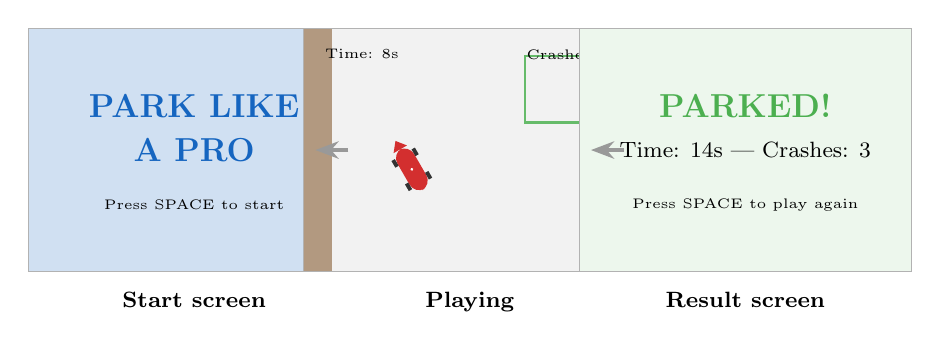
\begin{tikzpicture}[scale=0.7]
  % Start screen mockup
  \begin{scope}[shift={(-5,0)}]
    \draw[black!30,thick] (-3,-2.2) rectangle (3,2.2);
    \fill[titlebg!20] (-3,-2.2) rectangle (3,2.2);
    \node[font=\large\bfseries,titlebg] at (0,0.8) {PARK LIKE};
    \node[font=\large\bfseries,titlebg] at (0,0) {A PRO};
    \node[font=\tiny] at (0,-1) {Press SPACE to start};
    \node[font=\footnotesize\bfseries,below] at (0,-2.4) {Start screen};
  \end{scope}
  % Game screen mockup
  \begin{scope}[shift={(0,0)}]
    \draw[black!30,thick] (-3,-2.2) rectangle (3,2.2);
    \fill[roadgrey!20] (-3,-2.2) rectangle (3,2.2);
    \fill[wallbrown!50] (-3,-2.2) rectangle (-2.5,2.2);
    \fill[wallbrown!50] (2.5,-2.2) rectangle (3,2.2);
    \draw[parkgreen,thick] (1,0.5) rectangle (2.2,1.7);
    \begin{scope}[scale=0.7]
      \drawcar{-1.5}{-0.5}{30}
    \end{scope}
    \node[font=\tiny,anchor=north west] at (-2.8,2) {Time: 8s};
    \node[font=\tiny,anchor=north east] at (2.8,2) {Crashes: 2};
    \node[font=\footnotesize\bfseries,below] at (0,-2.4) {Playing};
  \end{scope}
  % Result screen mockup
  \begin{scope}[shift={(5,0)}]
    \draw[black!30,thick] (-3,-2.2) rectangle (3,2.2);
    \fill[grassgreen!10] (-3,-2.2) rectangle (3,2.2);
    \node[font=\large\bfseries,grassgreen] at (0,0.8) {PARKED!};
    \node[font=\footnotesize] at (0,0) {Time: 14s | Crashes: 3};
    \node[font=\tiny] at (0,-1) {Press SPACE to play again};
    \node[font=\footnotesize\bfseries,below] at (0,-2.4) {Result screen};
  \end{scope}
  % Arrows
  \draw[-{Stealth},very thick,black!40] (-2.2,0) -- (-2.8,0);
  \draw[-{Stealth},very thick,black!40] (2.8,0) -- (2.2,0);
\end{tikzpicture}
\end{center}

\begin{challengebox}
\begin{itemize}[nosep]
  \item Play 3 rounds. What's your best time?
  \item Try for 0 crashes AND a fast time --- speed vs.\ care!
  \item Show someone else. Watch them play. Is the game fun for them?
  \item What would you change to make it harder? Easier?
\end{itemize}
\end{challengebox}

\begin{stretchbox}
\begin{itemize}[nosep]
  \item Add more parking spots --- park in all of them to win
  \item Add a ``best time'' variable that remembers your record across rounds
  \item Create different course layouts for different levels
\end{itemize}
\end{stretchbox}

\newpage

% =============================================
% QUICK REFERENCE
% =============================================
\section*{Quick Reference: Scratch Blocks}
\addcontentsline{toc}{section}{Quick Reference}

\renewcommand{\arraystretch}{1.3}
\begin{tabularx}{\textwidth}{l l X}
\toprule
\textbf{Block} & \textbf{Category} & \textbf{What it does} \\
\midrule
\texttt{when green flag clicked} & Events & Starts the script \\
\texttt{when I receive} & Events & Starts on broadcast \\
\texttt{broadcast} & Events & Sends message to all sprites \\
\midrule
\texttt{go to x: y:} & Motion & Sets position \\
\texttt{point in direction} & Motion & Sets facing angle \\
\texttt{move (n) steps} & Motion & Moves forward/backward \\
\texttt{turn (n) degrees} & Motion & Rotates the sprite \\
\texttt{x position / y position} & Motion & Current position \\
\texttt{direction} & Motion & Current angle \\
\midrule
\texttt{forever} & Control & Loops forever \\
\texttt{if <> then / else} & Control & Checks a condition \\
\texttt{wait until <>} & Control & Pauses until true \\
\texttt{stop [all]} & Control & Stops everything \\
\midrule
\texttt{key pressed?} & Sensing & Is a key held down? \\
\texttt{touching [sprite]?} & Sensing & Sprite overlap check \\
\texttt{touching color?} & Sensing & Touching a colour? \\
\texttt{timer / reset timer} & Sensing & Built-in stopwatch \\
\midrule
\texttt{set / change variable} & Variables & Update stored numbers \\
\midrule
\texttt{join} & Operators & Combine text \\
\texttt{round} & Operators & Round a number \\
\texttt{abs of} & Operators & Distance from zero \\
\midrule
\texttt{show / hide} & Looks & Visible/invisible \\
\texttt{switch costume} & Looks & Change appearance \\
\texttt{say for secs} & Looks & Speech bubble \\
\texttt{go to front layer} & Looks & Put on top \\
\midrule
\texttt{start sound} & Sound & Play a sound effect \\
\bottomrule
\end{tabularx}

\vfill

% =============================================
% WHAT'S NEXT
% =============================================
\section*{What's Next?}
\addcontentsline{toc}{section}{What's Next?}

You've built a real game! Here are ideas if you want to keep going:

\textbf{Session 7: Reverse!}
Put the car in reverse gear. When speed is negative, steering works \emph{backwards} --- turning left makes the back go right. This is why reversing into a parking space is so tricky. Try adding parallel parking!

\textbf{Session 8: Traffic!}
Add other cars. Start with parked cars as obstacles. Then try making one drive back and forth. Now you have to time your moves!

\textbf{Session 9: Different Cars.}
What if the car was longer? Shorter? Longer cars are harder to park (bigger turning radius). Short cars are easier. Try making a stretched ``limo'' version and see the difference. That's physics in action.

\vspace{1cm}
\begin{center}
\textit{Made with curiosity and Scratch. Happy parking!}
\end{center}

\end{document}
